\section{Softwarearchitektur}

Nachfolgend wird die Softwarearchitektur mittels dem \gls{glos:c4} die Softwarearchitektur von blobfish dokumentiert.

\subsection{System context}

\begin{figure}[H]
    \centering
    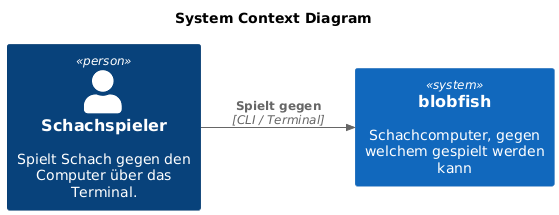
\includegraphics[width=\linewidth]{generated-diagrams/c4-context}
    \caption{Softwarearchitektur - System context}
    \label{fig:c4-context}
\end{figure}

Angefangen mit dem Systemkontext, ist zu erkennen, dass es sich oberflächlich um ein einfaches System handelt: Ein Schachspieler,
welcher anhand einer CLI gegen einen Schachcomputer, blobfish, Schach spielt.

Da die Applikation eine Java-Applikation ist, als \gls{glos:uberjar} ausgeliefert wird die Applikation ohne weitere \gls{glos:c4container}
auskommt, wurde auf das Container Diagram verzichtet, das keinen wirklichen Mehrwert gegenüber dem Context-Diagramm bietet,
da es praktisch dasselbe ist.

\subsection{Component}

\begin{figure}[H]
    \centering
    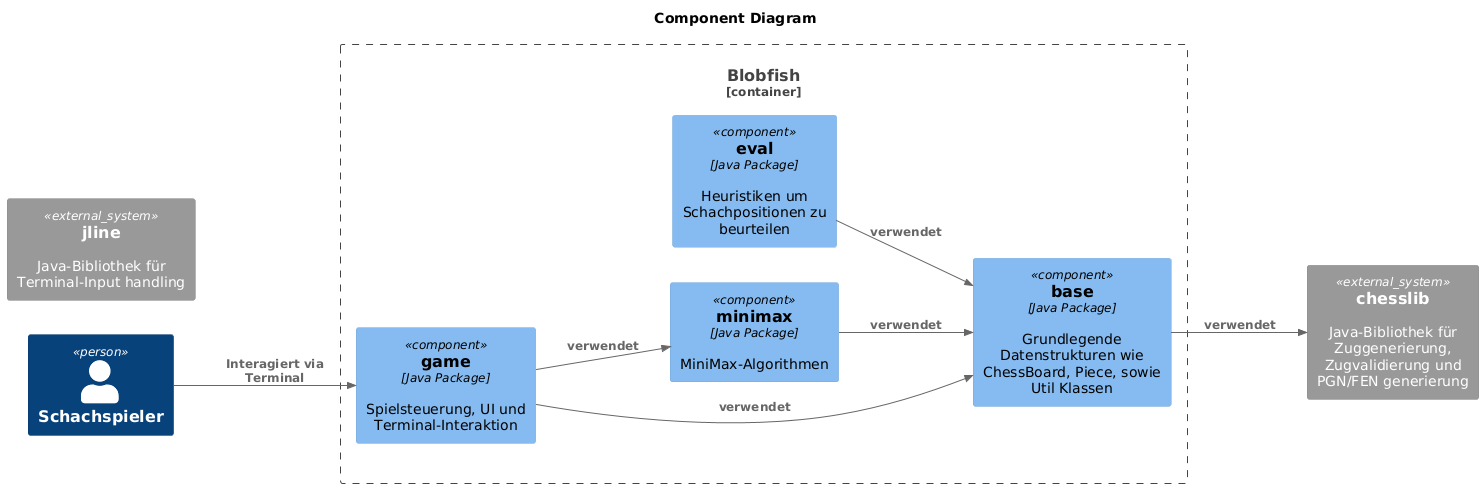
\includegraphics[width=\linewidth]{generated-diagrams/c4-component}
    \caption{Softwarearchitektur - Component diagram}
    \label{fig:c4-component}
\end{figure}

\subsection{Code}

\subsubsection{eval}

\begin{figure}[H]
    \centering
    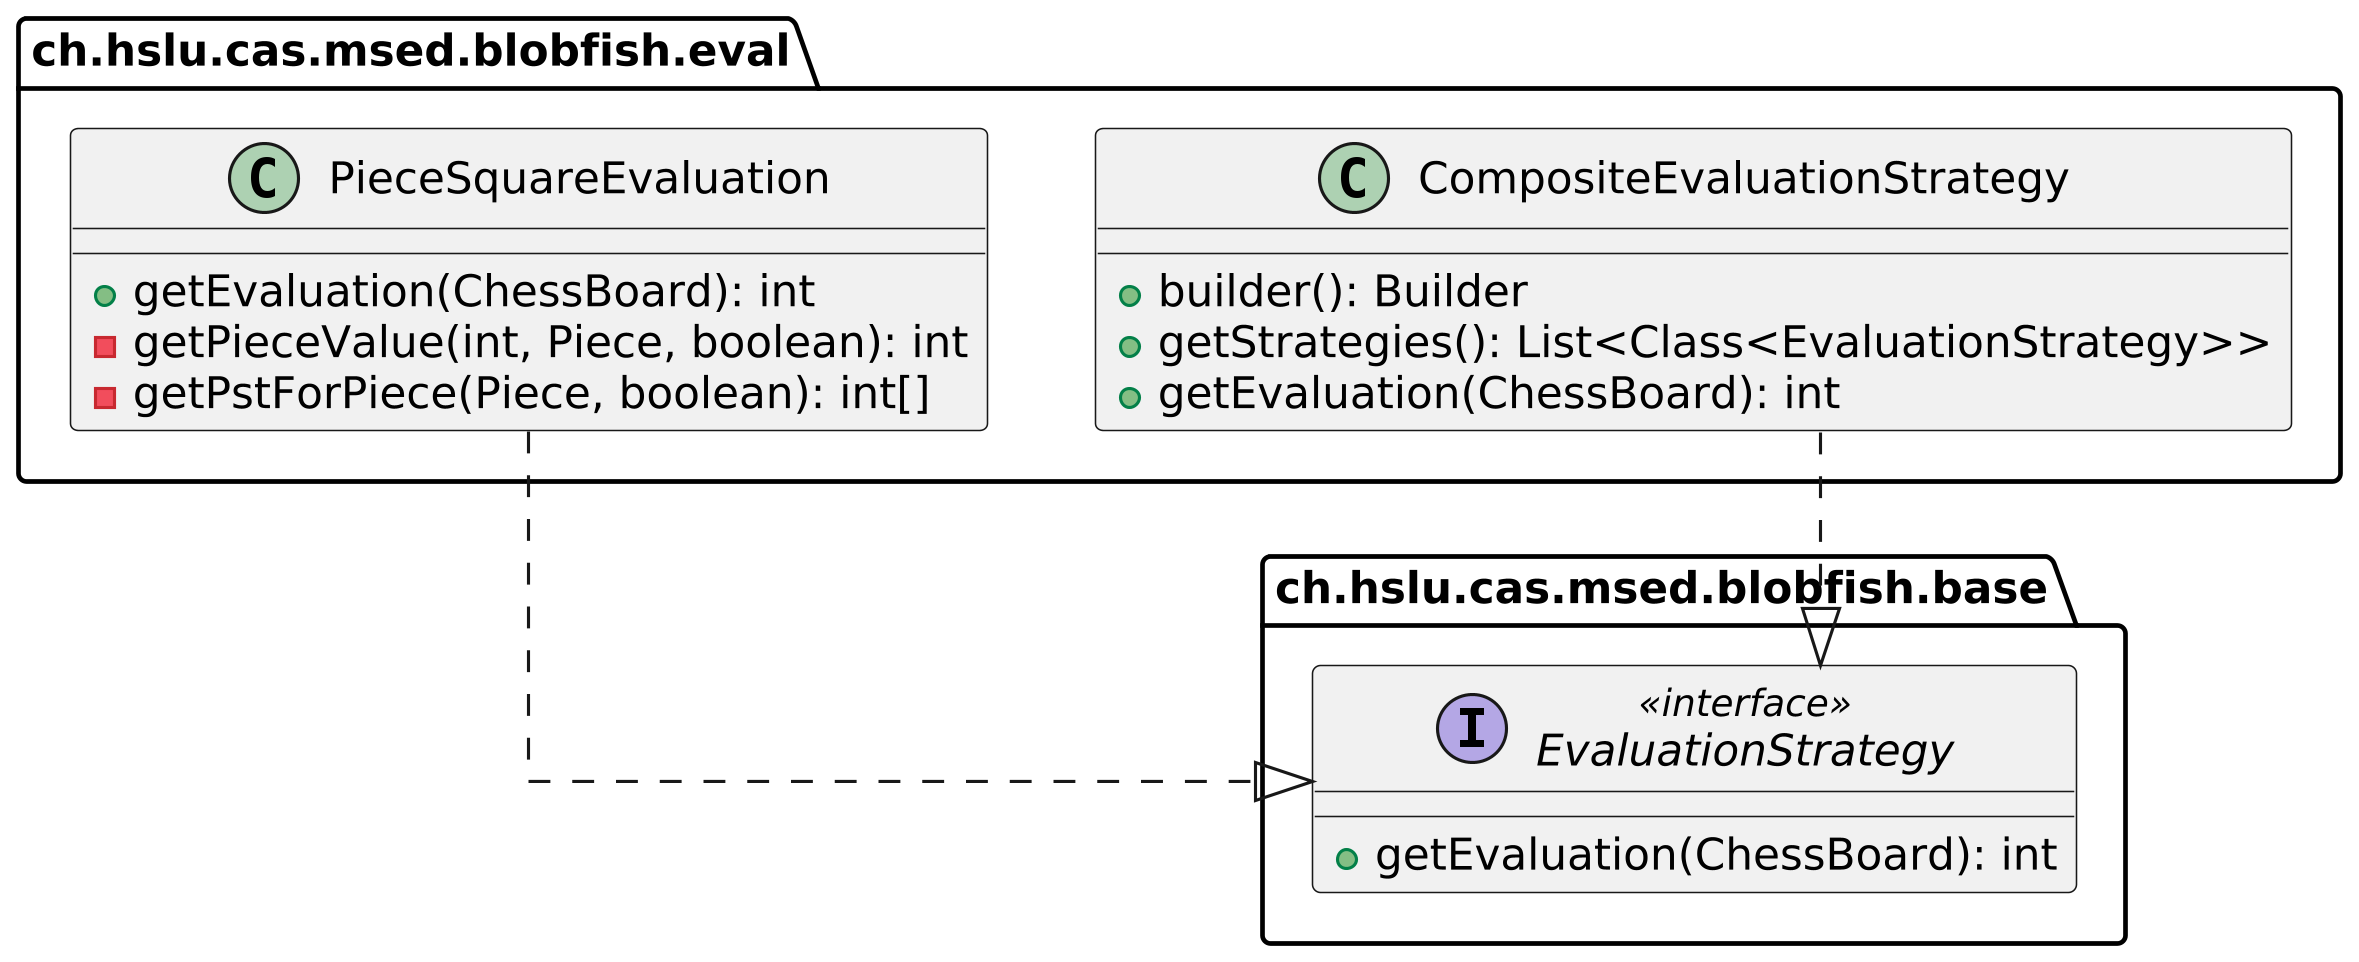
\includegraphics[width=\linewidth]{generated-diagrams/eval-code}
    \caption{Softwarearchitektur - eval}
    \label{fig:softwararchitecture-eval}
\end{figure}

\subsubsection{minimax}

\begin{figure}[H]
    \centering
    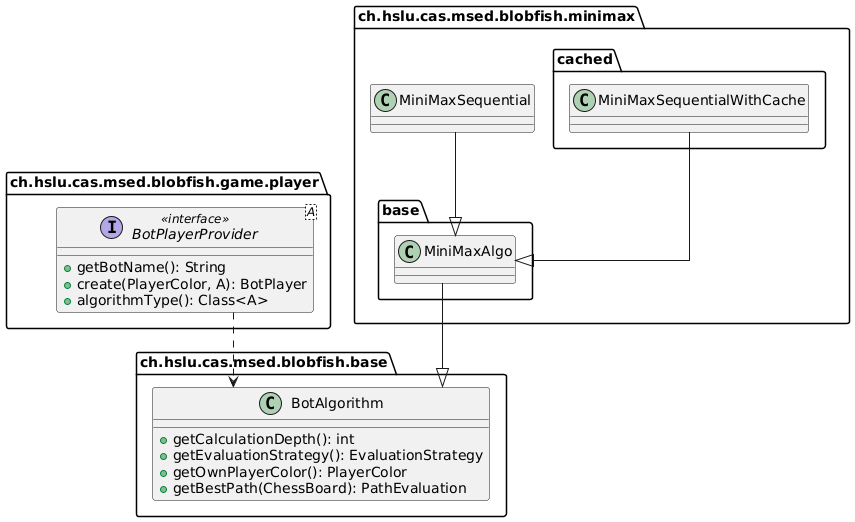
\includegraphics[width=\linewidth]{generated-diagrams/minimax-code}
    \caption{Softwarearchitektur - minimax}
    \label{fig:softwararchitecture-minimax}
\end{figure}